%\documentclass[12pt]{article}
\documentclass[espaco=simples,appendix=Name]{abnt}

\usepackage{abntex}
\usepackage[brazil]{babel}
\usepackage[T1]{fontenc}
\usepackage[utf-8]{inputenc}
\usepackage{hyperref}
\usepackage{times}
\usepackage{listings}
\usepackage[dvips]{graphicx}

\usepackage[num]{abntcite}      % citacoes do abntex
\usepackage{tabela-simbolos}    % tabelas de simbolos do abntex
\usepackage{dsfont}             % fonte
\usepackage{fancyvrb}


%\citeoption{abnt-full-initials=yes}
\lstset{language=ruby,caption=Exemplo,label=Ruby, numbers=left, frame=single} 

\title{Expressividade da linguagem enquanto programando}

\author{Jônatas Davi Paganini}

\date{novembro de 2009}

\begin{document}
\maketitle
\begin{abstract}
Este trabalho busca trazer ao leitor um ambiente de programação mais próximo de sua realidade. Através de exemplos de programas de computador, será mostrado como a linguagem de programação pode ser expressiva e de fácil compreensão. Com a linguagem Ruby, são abordados exemplos de uma linguagem de computador mais humana.
\end{abstract}

%\tableofcontents

\chapter{Teoria da linguagem}



Linguagem não é somente as línguas, mas é uma série de outros sistemas de comunicação, notação ou cálculo, criados artificialmente pelo homem com objetivos específicos. As linguagens de computador, arquitetadas para facilitar o trabalho do homem em traduzir o código de máquina, muitas vezes são complexas e de difícil aprendizado.

Apesar de ser um código com regras determinadas, natural ou artificialmente, as linguagens podem ser consideradas sobre um ponto de vista comportamental. \cite{linguagemLinguistica}

Portanto, pode se dizer que as linguagens possuem flexibilidade e versatilidade, sendo usadas através do interesse e da vontade humana. Isso se deve à produtividade dos sistemas de linguagem, que possibilitam a construção e interpretação de novos sinais. Todos os sistemas possibilitam a seus usuários construir e compreender um número indefinido de enunciados, que jamais viram antes. Isso, por outro lado, se dá dentro dos limites estabelecidos pelas regras.

As linguagens de programação estão sobre estes mesmos trilhos, conseguem ser flexíveis e estabelecer a definição de novos sinais e expressões. Este artigo abordará exemplos práticos de expressividade na programação, trará ao conhecimento do leitor uma forma produtiva de programar, analisando um domínio específico de as regras a partir de mini-linguagens internas de contextos específicos.


Os elementos constitutivos da linguagem são, pois, gestos, sinais, sons, símbolos ou palavras, usados para representar conceitos de comunicação, idéias, significados e pensamentos. Embora os animais também se comuniquem, a linguagem propriamente dita pertence apenas ao Homem. \cite{wikiLinguagem}

\chapter{Evolução da linguagem de programação}

A evolução dos computadores trouxe dispositivos menores e mais potentes. Na década de 80, usavam-se grandes computadores para realizar pequenos processos, 30 anos mais tarde estes dispositivos ganharam velocidade, design e consomem pouca energia. Dispositivos que cabem na palma da mão, com apenas alguns toques ou cliques tornam acessível a informação desejada. 

Da mesma forma, os computadores ganharam potência, as linguagens de programação se tornaram expressivas e humanas. Este dinâmismo não tem o objetivo de trazer conforto a máquina, mas sim ao seu manipulador - o homem. 

A linguagem de computador, inicialmente era grosseira e de difícil compreensão, com o passar do tempo, as técnicas foram evoluindo, ganhando forma e expressão. Houve uma percepção de mudança, que tornaria a linguagem de programação uma auxiliadora do programador e não uma interpretadora.

Uma linguagem tem os seus limites, na maioria dos casos é formal e burocrático. A linguagem Ruby quebra esta formalidade, torna o processo de codificação simples e livre. Em outras palavras, ela não bloqueia o trabalho do programador.

\section{Exemplo 'Hello world'}

   O programa Hello world é o programa mais conhecido no mundo inteiro e é o exemplo mais básico de uma linguagem de programação com o objetivo de imprimir a mensagem "Hello, world!" e guiar o iniciante em sua primeira compilação/execução de um programa de computador. Abaixo seguem dois exemplos "Hello, world" em duas linguagens de programação distintas: asssembly e ruby.


\subsection {Exemplo usando a linguagem de programação assembly}

Assembly ou Assembler é uma notação escrita por humanos que permite escrever instrução de máquina de forma mais fácil. Assembly paga o preço da complexidade pelo reduzido número de comandos e opções.

\begin{lstlisting}[label=exemplo em assembly,caption=Exemplo em assembly]
   variable:
      .message   db   "Hello world!\$"
   code:
      mov  ah,9
      mov  dx,offset .message
      int  0x21
      ret
\end{lstlisting}

Sem dificuldades, a listagem acima \ref{exemplo em assembly} demonstra-se complexa. Apenas para imprimir uma frase foram necessários 6 linhas. Essa declaração não tão amigável é usada para realizar o mesmo objetivo do comanddo abaixo \ref{exemplo hello world ruby}, apenas estão escritas de forma diferente. O fato é que os compiladores exigem uma quantidade mínima de declarações para que possa compilar e executar.


\subsection {Exemplo usando a linguagem de programação ruby}

\begin{lstlisting}[caption=Exemplo em ruby]
   print "Hello, world!"
\end{lstlisting}

 Ruby demonstra-se mais simples nestas exigências, é possível compilar apenas uma expressão, não precisando de declarações e nem padrões repetitivos. O código possuí apenas o comando de impressão e a frase que deseja ser impressa.

\section { A simplicidade da linguagem }

Foi necessário apenas uma linha de código para representar o mesmo exemplo na linguagem ruby. No exemplo mais simples o objetivo é apenas imprimir "Hello, world!" e é exatamente isso que está escrito. Diferente de assembly, ruby não é uma linguagem compilada e sim dinâmica. Assim, tudo acontece em tempo real, enquanto está sendo executado.
   
\begin{lstlisting}[caption=Tradução do programa ruby]
   imprima "Ola mundo!"
\end{lstlisting}

Apenas com uma linha de código é possível fazer exatamente o que está sendo proposto. Este programa de computador foi escrito de forma simples e humanamente legível, diferente da primeira instrução de máquina escrita em assembly. Com poucas palavras cumpriu exatamente o objetivo do software no domínio em questão.
Exemplos como este, mostram o poder do homem de categorizar e generalizar as informações. Desta forma a percepção mudou de, programar para o computador para programar para as outras pessoas. Anteriormente, com uma programação rígida e a escassez de processamento, a codificação de um software realmente fazia parte de um processo árduo e lento, onde não era possível tornar agradável a leitura de uma instrução de computador.

\section { A burocracia da linguagem }

Declarar e inicializar variáveis, importar pacotes, classes finais e fechadas são fatores que interferem no trivial desenvolvimento de software. As linguagens estáticas empurram o programador a escrever mais código, forçam a declarar estruturas sem sentido por não saber lidar com o problema com alto nível.

\begin{lstlisting}[label=HelloWorldJava, caption=Programa Hello World em Java]
 public class Hello {
     public static void main(String[] args) {
         System.out.println("Hello, World!");
     }
 }
\end{lstlisting}

Para ser possível executar um código em java, este código deve estar em uma classe Java, em um arquivo na extensão .java. A classe deve ser pública e deverá conter um método estático, sem retorno (\textbf{void}) com o nome \textbf main. Este método receberá como parâmetro um vetor de strings que representam os parâmetros da linha de comando. Para compilar o arquivo java, será necessário usar o compilador \textbf{javac} que então criará um arquivo com o mesmo nome do código fonte com a extensão .class, este arquivo pode ser executado usando o comando \textbf{java}. 
Todos estes passos devem ser seguidos sem falhas para que o exemplo hello world seja compilado e executado usando a linguagem java. Cada detalhe deste tem um motivo e é importante em algum aspecto na linguagem, mas em muitos momentos, estes recursos se tornam desumanos e complexos, obfuscando a expressividade da linguagem.

\chapter { A linguagem ruby }

Ruby é uma linguagem dinâmica, open source com foco na simplicidade e produtividade. Tem uma sintaxe elegante de leitura natural e fácil escrita. Com um grande número de bibliotecas disponíveis gratuitamente (gems), tem atraído muita gente para desenvolver nesta linguagem.

Para usar no Mac OS X ou Linux, é necessário abrir o {Terminal ou Console} e no Windows pode-se usar o Command-DOS e após isso digitar ruby.exe para invocar o compilador, irb para iniciar uma interação.


\section { O compilador ruby }

Ruby é uma linguagem de script, dinâmica e compila em tempo de execução. O mesmo compilador que compila o código também executa. O compilador pode ser invocado usando a linha de comando e receber código por parâmetro compilar

\begin{lstlisting}[caption=Usando o compilador na linha de comando]
jonatas@xonatax-mac:~$ ruby -e "puts 1+2"
3
\end{lstlisting}

Também é possível escrever um arquivo ou vários

\section { Ruby Interativo - IRB }

Existe um programa chamado IRB, que vem instalado com compilador de ruby, que serve para interagir com a linguagem na forma de console. As linhas do console ruby digitadas são iniciadas por \textbf{>>} e as linhas que trazem o resultado da expressão são iniciadas por \textbf{=>}. Estes símbolos quando exibidos no início da linha, não fazem parte do código de programação, apenas identificam a situação do terminal interativo.

\begin{lstlisting}[caption=Usando o compilador na linha de comando]
jonatas@xonatax-mac:~$ irb
>> 1.class
=> Fixnum
>> 1 + 2
=> 3
\end{lstlisting}

\section { Tipos de dados }

Tudo em ruby é um objeto, todas as classes são abertas e podem ser alteradas ou extendidas. A seguir serão abordados os tipos básicos de dados para trabalhar com ruby.

\subsection { Strings }

As strings podem ser limitados por vários delimitadores, em geral são usadas aspas simples e duplas, mas existem outras formas. Uma string é um dado que contem uma informação em formato texto. Em ruby é encarado como uma cadeia de caracteres, e pode ser também fácilmente manuseado como um vetor de caracteres.

\begin{lstlisting}[caption=Exemplos de uso de string]
>> " outra string" + ' mais uma' + %[ outra ]
=> " outra string mais uma outra "
\end{lstlisting}

\subsection { Números }

Os números são objetos como qualquer outro e os operadores são simples métodos.

\begin{lstlisting}[caption=Exemplos de uso de números ]
>> 1.class
=> Fixnum
>> 1.class.ancestors
=> [Fixnum, Integer, Precision, Numeric, Comparable, Object, Kernel]
>> 1.0.class
=> Float
\end{lstlisting}

\subsection { Hashes }

Este tipo de elemento que amarzena valores como uma matriz, mas é possível acessar os valores através de uma chave. O valor do elemento é indicado apartir da expressão:

\begin{lstlisting}[caption=Syntaxe do hash]
{ :chave => valor }
\end{lstlisting}

Tanto chave quanto valor podem ser objetos de qualquer tipo. Lembrando que a chave é a forma de acessar um valor, logo não poderá haver chaves iguais na mesma estrutura. 

\begin{lstlisting}[label=exemplohash, caption=Exemplos de uso de hashes]
sexo = { "M" => "Masculino", "F" => "Feminino"}
sexo["M"] # => "Masculino"

pessoa = { :nome => "jonatas", :idade => 22, :cpf => "047..." }
pessoa[:rg] # => nil
\end{lstlisting}

Quando invocada uma chave que não existe, a expressão retorna \textbf{nil} ou \textbf{nulo}. \textbf{Nil} também é um objeto em Ruby, e é um objeto falso, o que auxilia no tratamento de excessões simples como requerir o documento de cpf ou rg da variável pessoa declarada acima\ref{exemplohash} :

\begin{lstlisting}[caption=Exemplos de uso de hashes com operador ou ]
documento = pessoa[:rg] || pessoa[:cpf] # => "047..."
print "sem documento!" if documento.nil?
\end{lstlisting}

No caso acima, quando não houver rg, irá buscar por cpf e atribuir ao documento. Se não encontrar nenhum dos dois então irá imprimir a mensagem avisando a falta do documento.

\subsection { Entrada de dados }

No exemplo abaixo será feito uma pergunta para o usuário e quando ele confirmar a resposta irá saudar o usuário.

\begin{lstlisting}[caption=Exemplo de entrada de dados ]
 print "qual seu nome?"
 nome = gets
 print "oi #{nome}"
\end{lstlisting}
 
Na primeira linha, é impressa a pergunta. Na próxima linha é atribuido a uma variável nome a entrada de dados dada pelo método gets.
Em seguinda é impressa a saudação juntamente com a variável nome. O uso da interpolação \#\{\} embutido na string concatena o resultado da expressão interna invocando o método to\_s(transforma em string).

\subsection { Métodos }

Os métodos podem ser usados apartir de uma classe, ou estarão definidos na classe Object que é a classe mais grande. Métodos são formas de interagir com o ambiente atual e encapsulam a função com parâmetros. Eles podem pertencer as classes ou as instâncias, 

\begin{lstlisting}[caption=Exemplo de método ]
def ligar_para(telefone)
  puts "ligando para #{telefone}"
end
\end{lstlisting}

\subsection { Classes e Módulos }
 
Classe é a declaração que permite definir uma classe marcado pela palavra \textit{class} seguido do nome de elementos. Após isso, vem o corpo com as definições do corpo. O fim do corpo é marcado pela palavra end.

Módulos permitem dividir comportamentos de classe e de instância, permitindo assim a multipla extensão de classes. Ele pode ser usado em blocos e sub-blocos e todo o código gerado fica encapsulado na declaração. Esse recurso também pode ser usado para agrupar classes do mesmo gênero. 

\begin{lstlisting}[caption=Exemplo de módulo ]
  module Mamifero
    def mamar
      print "mamando..."
    end
  end
  class Gato
    include Mamifero
    def miar
       print "meauuuu"
    end
  end
\end{lstlisting}

Os módulos também são uma boa possibilidade para criar espaços de nomes. Com este recurso é possível trabalhar com nomes específicos e sem repetições de nomes.

No exemplo acima, é definido um módulo Mamifero está sendo declarado os seus recurso internos. Um módulo não pode ser instanciado, ele é apenas usado como um espaço de nomes. O objetivo dele é organizar pequenos comportamentos que podem ser utilizados em outros momentos.

\begin{lstlisting}[caption=Exemplo de módulo como espaço ]
module Condominio
  include PortaoEletronico
  class Apartamento
   # ... define o apartamento internamente
  end
end 
\end{lstlisting}

\subsection{ Variáveis } 

Quando iniciados com apenas um arroba (@), indicam ser uma variável de instância. Diferente de Java e muitas outras linguagens, não é necessário declarar a variável antes de usa-la. Elas simplesmente criam a referência logo na primeira vez que são usadas.
As variáveis locais são iniciadas por letras ou \textit{underscore}.
A atribuição de um valor a uma variável é feita através do sinal de igualdade (=).

\begin{lstlisting}[caption=Exemplo de variável local ]
meu_nome = "Jonatas"
\end{lstlisting}

A leitura da expressão acima seria: meu nome (a variável) é igual a Jonatas.
Em uma classe, as váriaveis são usadas como atributos internos.

\begin{lstlisting}[caption=Exemplo de variável de instância em uma classe ]
class Pessoa
  def initialize(nome)
    @nome = nome
  end
  def saudar
    puts "ola #{@nome}"
  end
end
\end{lstlisting}

O código anterior declarou a classe que pode ser utilizada da seguinte forma:

\begin{lstlisting}[caption=Exemplo de utilização da classe descrita acima ]
jonatas = Pessoa.new "Jonatas"
jonatas.saudar 
\end{lstlisting}

\subsection { Blocos de código }

\cite{programmingRuby}
Segundo Dave Thomas, todo mundo já quiz implementar o seu próprio recheio de método na sua própria estrutura. Um bloco pode ficar entre chaves ou entre as palavras \textit{ do } e \textit{ end }.

\begin{lstlisting}[caption=Exemplo de bloco de código ]
   5.times { print "hello word" }
\end{lstlisting}

Traduzindo: 
\begin{lstlisting}[caption=Exemplo de bloco de código ]
   5.vezes { imprima "ola mundo" }
\end{lstlisting}

O bloco de código é extensamente utilizado em \textit{frameworks} para apenas criar a estrutura e tornar óbvio o objetivo da linguagem.


\chapter{ Shoes }

\section{O que é Shoes?}

Shoes é um framework para a construção de interfaces rápidas. Shoes nasceu pra ser fácil. Realmente feito para iniciantes absolutos. Com esta ferramenta é realmente fácil de fazer interfaces e artes gráficas. 
Esta ferramenta permite criar interfaces desktop para todas as plataformas e muitos divertidas de aprender.

\section{ Primeiro exemplo }

Este é um dos exemplos mais simples do shoes. 

\begin{lstlisting}[caption=Primeiro exemplo do framework Shoes  ]
Shoes.app { 
  button("Click me!") {
     alert("Good job.") 
  }
} 
\end{lstlisting}

Este programa foi escrito em uma linguagem chamada Ruby. Consiste em uma janela com um botão. Quando o botão for clicado ela deverá responder por: "Good job." ou seja "Bom trabalho."

Shoes roda na maioria das plataformas operacionais. Isto é ótimo pois é possível escrever apenas uma vez e usar no Linux, Mac OS X, Windows e muitos outros.

%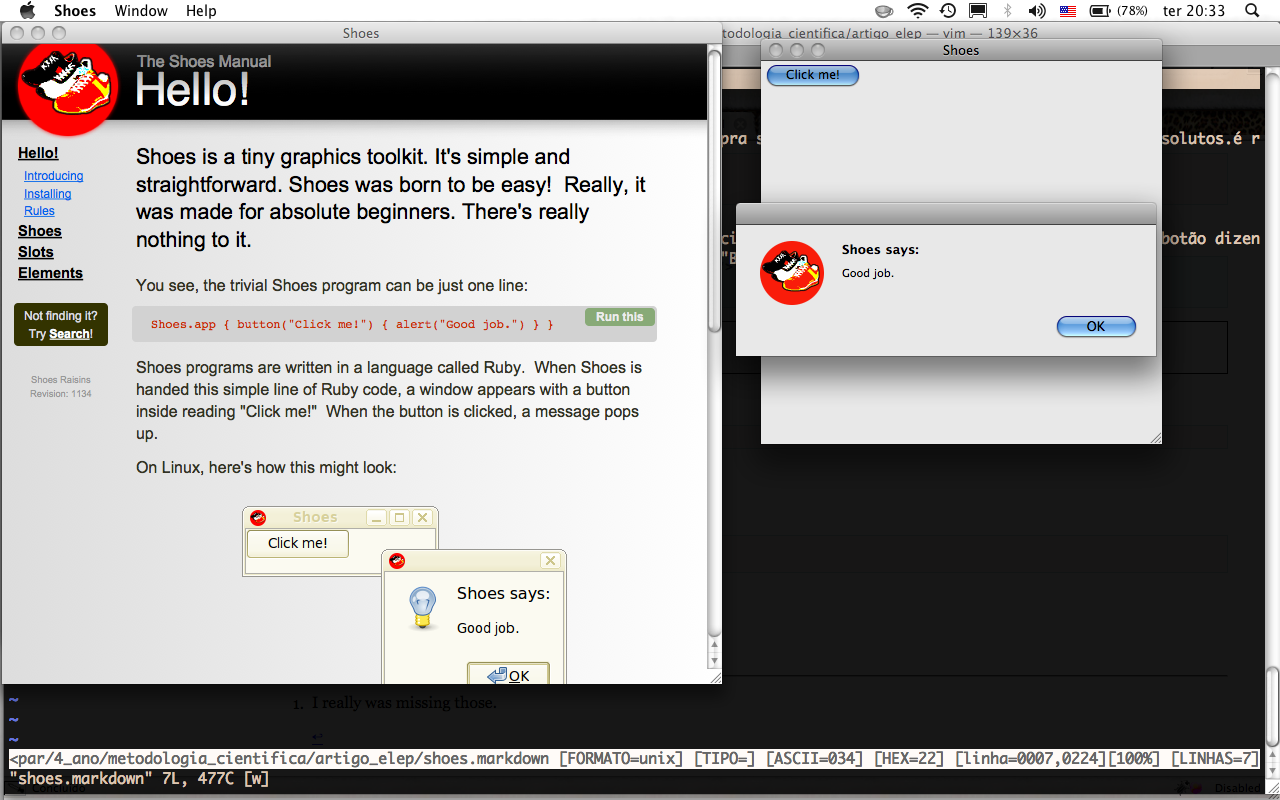
\includegraphics[scale=0.6]{shoes_hello_world.eps}
% (exemplo rodando no Mac OS X)!

\subsection{ Exemplo de expressividade - um bloco de notas com Shoes }

Como próximo exemplo, será progamado um bloco de notas que possa apagar e inserir novas notas em uma janela. O programa será composto por:
\begin{itemize} 
  \item uma janela com um título "Minhas Notas", largura de 300 pixels. E dentro desta janela terá 
  \begin{itemize} 
    \item uma linha de edição para escrever a nota
    \item um botão para adicionar a anotação que quando for clicado deve 
    \begin{itemize} 
      \item adicionar o que foi escrito na linha de edição para as notas abaixo listadas
      \item limpar o texto da linha de edição da nota
    \end{itemize} 
  \end{itemize} 
  \item cada nota adicionada deve conter um link para remover a nota \ldots
\end{itemize} 


\subsection { Funcionamento do framework }

Como descrito na primeira linha de código do exemplo anterior, o framework é declarado, contendo uma janela principal. Esta janela, recebe um título e um tamanho inicial.
A declaração:

\lstinputlisting[caption=Um bloco de anotações com Shoes]{shoes_tarefas.rb} 

Shoes.app inicia um aplicativo do framework, e dentro do corpo deste método é possível empilhar e enfileirar objetos. Com suas definições específicas de janela, também pode receber parâmetros. Este objeto pode encaixar muitos outros componentes internamente. Também é possível manipular elementos de fora para dentro, e de dentro para fora, fazendo com que um bloco interfira no outro sem dificuldades.

Como o exemplo acima mostra, o framework Shoes basicamente é uma pilha de componentes, podendo adicionar, empilhar e remover elementos com facilidade e clareza. Estes elementos quando empilhados, podem interagir apenas empilhados ou empilhados e aninhados a outras pilhas de elementos. 


\lstinputlisting[firstline=1, lastline=1, caption=Primeira explicação do framework Shoes]{shoes_tarefas.rb} 

Estes parâmetros como título(title) e tamanho(width) são pertencentes a janela principal do aplicativo, e podem ser acompanhados de outros como bloqueio de redimensionamento de janela.

Os parâmetros no formato chave e valor facilitam o uso e a extensão das possibilidades para cada elemento. Infinitamente podem trabalhar com novas funcionalidades e com os valores padrões.

Na segunda linha do código existe a declaração do elemento da interface edit\_line que é responsável pela linha de edição que permite a entrada de dados.
\lstinputlisting[firstline=2, lastline=2, caption=Entendendo a linha de edição]{shoes_tarefas.rb} 

Este método edit\_line retorna um componente do Shoes do tipo caixa de entrada de texto, e é possível acessar o valor do texto digitado através do atributo text. 

\lstinputlisting[firstline=3, lastline=9, caption=Entendendo o botão e sua ação]{shoes_tarefas.rb} 

No fragmento acima, é declarado o botão que faz. Muito semelhante a especificação do programa Shoes proposto, este fragmento cumpre a seguinte parte: 

\begin{itemize} 
  \item adicionar o que foi escrito na linha de edição para as notas (linhas 5 e 6)
  \item cada nota adicionada deve conter um link para apagar a nota (linha 6)
  \item limpar o texto da linha de edição da nota (linha 8) \ldots
\end{itemize} 

Traduzindo na literal a declaração do botão:

\begin{lstlisting}[caption=Botão adicionar - código traduzido]
  botao "adicionar" {  
    @notas.adicionar { 
      paragrafo(@anotacao.texto + " " + 
          link("apagar") {|nota| nota.pai.remover })
    }  
    @anotacao.texto = ""
  } 
\end{lstlisting}

Um botão adicionar \textbf{(botao "adicionar")} que faz com que, o texto da anotação \textbf{(@anotacao.texto)} seja adicionado em baixo das notas \textbf{(@notas.adicionar)} já existentes. Quando clicado no link de apagar \textbf{(link("apagar"))} aquele elemento \textbf{(nota)}, ele referencia-se a seu pai que o remove como filho \textbf{(nota.pai.remover)}, desaparecendo da pilha de anotações \textbf{(@notas)}.

\lstinputlisting[firstline=10, lastline=10, caption=Entendendo a pilha de notas]{shoes_tarefas.rb} 

Traduzindo na literal a linha 10:

\begin{lstlisting}[caption=Entendendo a pilha de componentes]
  @notas = pilha :margem => 20, :largura => 300
\end{lstlisting}

A váriavel \textbf{@notas} é igual a uma pilha de componentes shoes com margem de 20 pixels e largura de 300 pixels. Esta pilha não exibe nada na tela até que não seja adicionado nenhum elemento nela. Quando o botão adicionar for pressionado então ela é usada para adicionar o texto escrito na nota. Observe que foi usado a variável em um bloco de código antes mesmo de ela existir. Se o botão for clicado antes da pilha de notas ser criada, então o sistema lançará uma merecida excessão. 

Shoes trabalha com pilhas e fluxos (\texttt{ stacks and flows }), esse conceito permite empilhar elementos e criar fluxos com outros. Eles não se misturam mas podem interagir. A pilha criada foi atribuida a váriavel \textbf{ @notas } e foi definido uma margem e uma largura para esta pilha de elementos. O processo pode funcionar recursivamente dentro desta pilha permitindo criar o mesmo fluxo interno e concatenar elementos com liberdade.

\chapter { Linguagens de domínio específico }

No domínio específico de construir telas o framework tem características que ressaltam a sua expressividade. A simplicidade de fazer um botão ter uma ação é expressiva no domínio de construir um botão com uma mensagem de alerta é muito semelhante ao exemplo a seguir\ref{exemplo botao}. Se é um botão, consequentemente terá uma mensagem e uma ação.  Em uma linha de edição (\textbf{edit\_line}) terá exatamente as propriedades de uma entrada de texto. 


\begin{lstlisting}[label=exemplo botao, caption=Simplicidade do botão]
botao("mensagem") { alerta("clicou no botao" } 
\end{lstlisting}


Para desenhar uma linguagem de domínio específico deve-se olhar para a forma mais fácil de expressar-se naquele contexto.
Cada elemento, em seu domínio específico tem a sua forma de expressão. Por exemplo,  existem várias opções para construir uma janela, esses elementos podem ser descritos através dos parâmetros do comando. Uma janela pode ter um título, um tamanho inicial, ser redimensionável, etc.

\begin{lstlisting}[label=exemplo janela, caption=Expressividade da construção de uma janela]
janela :largura => 300, :altura => 500, 
       :titulo => "Janela de exemplo" {

  botao("exemplo")
}
\end{lstlisting}


Cada problema, no seu contexto, pode ser expressivo quando usando uma terminologia adequada para o domínio específico. A maioria das linguagens de programação dificulta a criação desta sintaxe dentro da própria linguagem. Ruby trabalha com estas linguagens de forma mais transparente. Leandro Heuert\cite{dslLeandro}, abordou o exemplo da criação de uma receita de bolo no seu domínio específico da seguinte forma: 

\begin{lstlisting}[label=exemplo receita, caption=Expressividade de uma receita no seu domínio específico\cite{dslLeandro}]
receita {
  nome "Bala de Pinga"
  ingrediente 1, 'kg', 'acucar cristal'
  ingrediente 1, 'copo', 'pinga'
  ingrediente 2, 'copos', 'agua'
  ingrediente 2, 'envelopes', 'gelatina incolor'
  ingrediente 1, 'envelopes', 'gelatina vermelha'
}
\end{lstlisting}

Os domínios específicos tornam o código estético e preciso. Yukihiro Matz Matsumoto, o criador da linguagem Ruby, pergunta em uma entrevista a Dave Thomas se as linguagens influenciam o ser humano. Ele discute o que é uma boa linguagem de programação. O que proporciona na maneira de pensar, como o faz um programador melhor. Sendo japônes, logo pensa em japônes mas tem que traduzir para inglês a sua forma de pensar. Ele argumenta que não existe uma maneira de programar em japônes, a linguagem simplesmente não permite, essa não seria uma boa linguagem para explorar como uma linguagem de programação. As linguagens devem fazer você pensar melhor e faze-lo um melhor programador.\cite{programmingRuby}

Em outra entrevista muito divertida \cite{entrevistaDivertidaComMatz} com Matz, ele comenta sobre a importância de aprender vários tipos de linguagem de programação. Para entender a produtividade que a linguagem pode oferecer, é necessário conhecer os bons aspectos das linguagens de script, funcionais, lógicas, etc. Aprender linguagens é uma maneira de aprender a programar. Ler códigos fontes é uma maneira de obter conhecimento e informação. Também não deve-se dar foco em ferramentas, pois elas mudam. O importante é conhecer a base fundamental dos algorítmos.

Ser preguiçoso é uma fonte de inspiração para programar em Ruby, as máquinas servem os homens e a elas pertence o esforço. Falando pouco e se expressando bem é possível comandar computadores com produtividade.

Heuert\cite{dslLeandro} conclui que quanto mais conhecido é o domínio específico, melhor será a solução. Uma linguagem pode ser desenhada com sucesso para um determinado escopo, pode ser comunicativa para as pessoas e para os computadores e expressiva como os exemplos aqui apresentados.

A atividade de trabalhar com a linguagem, uma forma de se comunicar com a máquina, deve ser divertida, e em primeiro lugar de homem para homem, depois de homem para máquina e por fim de máquina para máquina\cite{entrevistaDivertidaComMatz}. Em outras palavras deve iniciar por uma definição compreensiva ao homem, depois deve ser comunicado para a máquina de forma fácil, e por fim a máquina pode compreender e se preocupar com suas tarefas de máquina.


Com uma linguagem bem desenhada, como Heuert citou "pode-se facilmente que pessoas que tenham um mínimo necessário de conhecimento em linguagens de programação consigam entender o quê está acontecendo por trás de um software"\cite{dslLeandro}. Trabalhando com elementos conhecidos na contexto do programador, é possível que mesmo sendo um iniciante, codifique sem dificuldades, já que conhece o domínio específico.

A metaprogramação é o poder de estender a linguagem a partir da própria linguagem. Dave Thomas\cite{programmingRuby} ressalta que uma das coisas que mais chama atenção em Ruby é a facilidade de instrospecção à linguagem. Com este recurso é possível criar objetos dinâmicamente, é possível trabalhar com o inesperado criando métodos e classes dinâmicamente, através da própria linguagem. Também é este o recurso que mais auxilia na definição do domínio específico da linguagem a ser desenhada. 



\bibliographystyle{plainat}
\begin{thebibliography}{9} 
\bibitem{wikiLinguagem} 
Wikipédia, 
Acesso em setembro de 2009.

\url{http://pt.wikipedia.org/wiki/Linguagem}

\bibitem{programmingRuby} 
Thomas, D. 
Programming Ruby: The Pragmatic programmers’ Guide. 
Segunda edição. Dallas, Texas: The Pragmatic Bookshelf, 2006.

\bibitem{dslLeandro} 
HEUERT, L. 
Linguagens Específicas de Domínio: um exemplo prático em Ruby.
Francisco Beltrão: UNIPAR, 2008.

\bibitem{entrevistaDivertidaComMatz}
Ruby Creator Y. Matsumoto.
Interview by S. Ibaraki, I.S.P.
\url{http://www.stephenibaraki.com/rubycreater122101.htm}

\bibitem{entrevistaAudioComMatz}
Matsumoto, Y.
Ruby Design Principles
Technometria with Phil Windley, 
Acesso em novembro de 2009.
%(Entrevista de audio em inglês). 
\url{http://itc.conversationsnetwork.org/shows/detail1638.html}

\bibitem{cantWriteAExpressiveCode}
Gageot, D.
We can’t write expressive code,
Acesso em novembro de 2009.
\url{http://blog.javabien.net/2009/01/12/can-we-really-write-expressive-code}

\bibitem{rubyPhilosophy}
Venners, B. The Philosophy of Ruby
A Conversation with Yukihiro Matsumoto
Acesso em novembro de 2009.

\bibitem{linguagemLinguistica}
Lyons, J.
Linguagem e Linguística,
Inglaterra: Universidade de Sussex, 1981.
% Tradução
% Marilda Winkler Averbug

\end{thebibliography} 

\end{document}


